\chapter{Schematic culvert test case}
%

% - Purpose & Problem description:
%     These first two parts give reader short details about the test case,
%     the physical phenomena involved and specify how the numerical solution will be validated
%
\section{Purpose}
%
The purpose of this case is to test the culvert functionality in TELEMAC-3D, qualitatively checking that
the behaviour of the flow between a tide-controlled river and a floodplain is consistent.

\section{Description}
%
This schematic test case consists of a piece of flood plain and a piece of tidal river
from an estuary and they are separated by a dike.
There is water exchange between the floodplain and the estuary through two culverts.
In normal tidal conditions the tide can enter the floodplain and this will create tidal nature like mud flats and marshes.
In storm conditions the culverts are closed and the floodplain is used as a buffer to store water.
The crest level of the dike between the estuary and the floodplain is a little lower than the other dikes containing the estuary.
When extreme high water levels occur inside the estuary, water can flow over the dike into the floodplain.
In this schematic test case we only want to simulate the exchange of water between estuary and floodplain through two culverts.

The floodplain has a bed level of 1m (TAW = Belgian reference level where 0m is about mean low water level).
The dike has a crest level of 6m and the estuarine river has a bed level of -5m.
An overview of the configuration is given in Figure \ref{fig:culvert_figure1}.
On the right side, the river side, a liquid boundary is set and a tidal signal
(i.e. a measured tidal signal from tidal gauge at Schoonaarde, Belgium in the Scheldt estuary)
in the form of water levels is applied.
Two nodes in the estuary communicate with two nodes in the floodplain to represent the two culverts.
One culvert allows flow in both directions and the other culvert only allows flow from the floodplain back to the estuary
(this type of culvert in the Scheldt estuary always has a one-way valve and makes sure flood water can return to the estuary after a storm surge).

\begin{figure}[h]
\begin{center}
	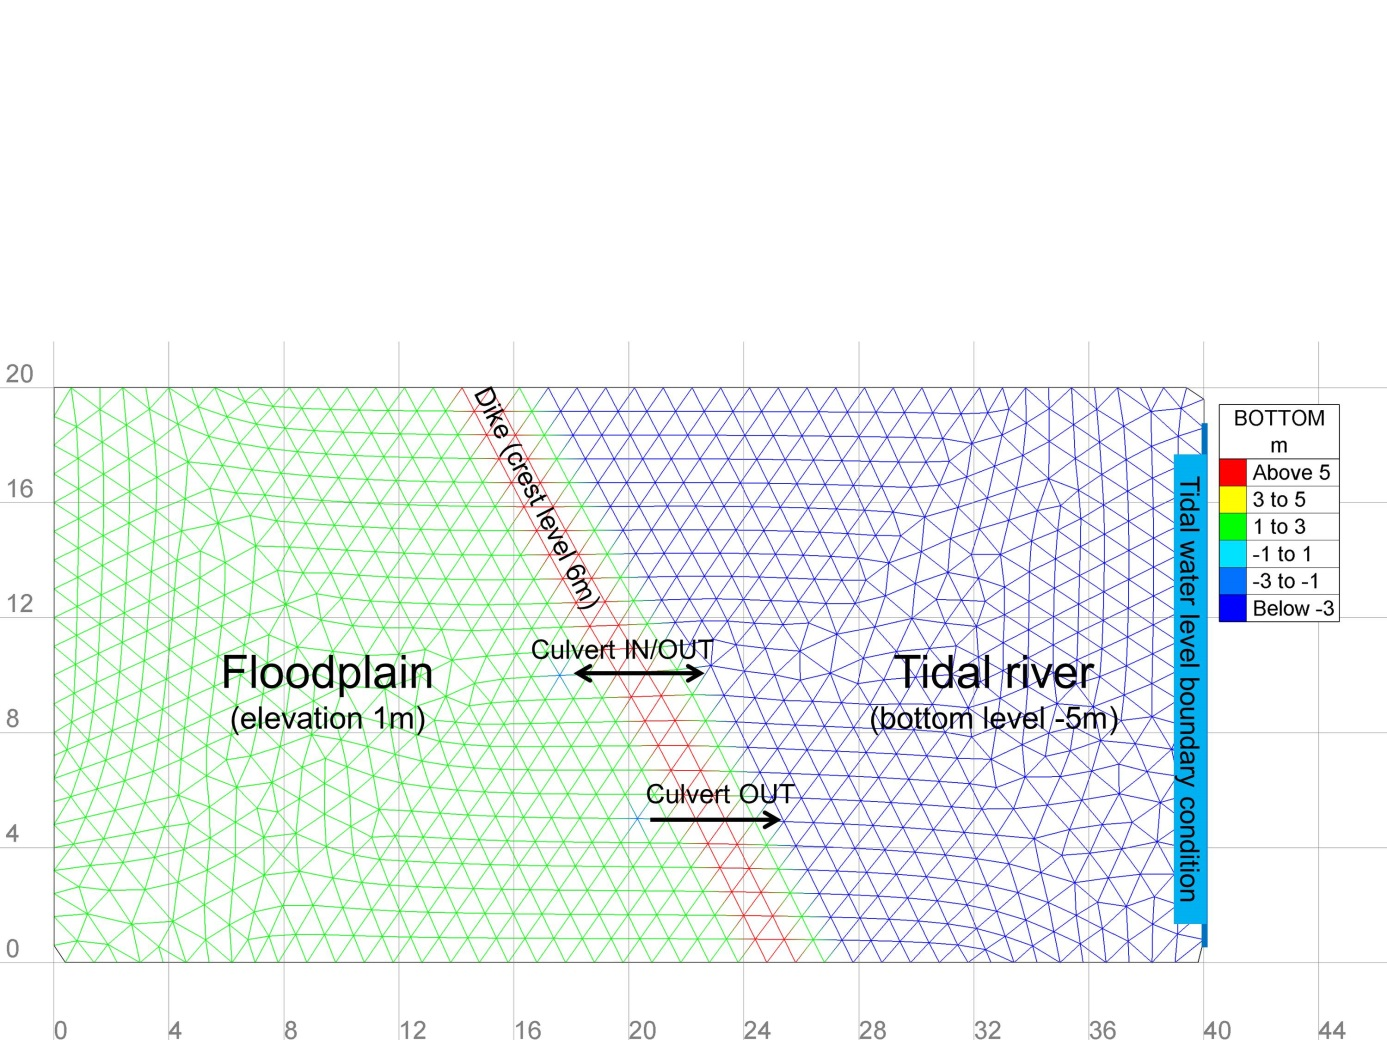
\includegraphics[scale=0.5]{img/figure1.png}
\end{center}
\caption{Overview of schematic test case for culvert testing}
\label{fig:culvert_figure1}
\end{figure}

\section{Computational options}
%
% - Mesh:
%     This part describes the mesh used in the computation
\subsection{Mesh}

\subsection{Initial and boundary conditions}
The water level in the river is prescribed through tidal boundary conditions.
%
% - Numerical parameters:
%     This part is used to specify the numerical parameters used
%     (adaptive time step, mass-lumping when necessary...)
\subsection{Numerical parameters}


The simulation time is about 28 hours.
The time step is set to 1 second, providing, together with the chosen mesh resolution, a stable simulation.

The bottom friction is taken into account in the model through the Manning Strickler’s parameter $n$, set to $0.02 s.m^{-1/3}$.
The horizontal and vertical turbulence viscosity coefficients are both set to $0.01 m^2s^{-1}$.

\subsection{Culvert characteristics}
The characteristics of the culverts are presented in Table \ref{tab:culvert_table1}.

\begin{table}[H]
\caption{Culvert specifications (these are as similar to the real field culverts as possible).}\label{tab:culvert_table1}
\begin{center}\begin{tabular}{|c|c|c|}
\hline
~ & \textbf{Culvert 1} & \textbf{Culvert 2} \\
\hline
\textbf{I1} & 583 & 637 \\
\hline
\textbf{I2}	& 432	 & 497 \\
\hline
\textbf{CE1}	& 0.5	 & 0.5 \\
\hline
\textbf{CE2}	& 0.5	 & 0.5 \\
\hline
\textbf{CS1}	& 1	 & 1 \\
\hline
\textbf{CS2}	& 1	 & 1 \\
\hline
\textbf{LRGbus}	& 1	 & 2 \\
\hline
\textbf{Haut1}	& 1.9	 & 1.5 \\
\hline
\textbf{CLP}	& 0	 & 2 \\
\hline
\textbf{LBUS}	& 0.2	 & 0.2 \\
\hline
\textbf{z1}	& 4	 & 1.5 \\
\hline
\textbf{z2}	& 4.7	 & 1.5 \\
\hline
\textbf{CV}	& 0	 & 1 \\
\hline
\textbf{C56}	& 10	 & 10 \\
\hline
\textbf{CV5}	& 1.5	 & 1.5 \\
\hline
\textbf{C5}	& 6	 & 6 \\
\hline
\textbf{Ctrash}	& 0.8	 & 0.1 \\
\hline
\textbf{Haut2}	& 1.2	 & 1.5 \\
\hline
\textbf{Fric}	& 0.015 & 0.015 \\
\hline
\textbf{Length}	& 13	 & 40 \\
\hline
\textbf{circ}	& 0	 & 0 \\
\hline
\end{tabular}\end{center}
\end{table}

\section{Results}

\begin{figure}[h]
\begin{center}
	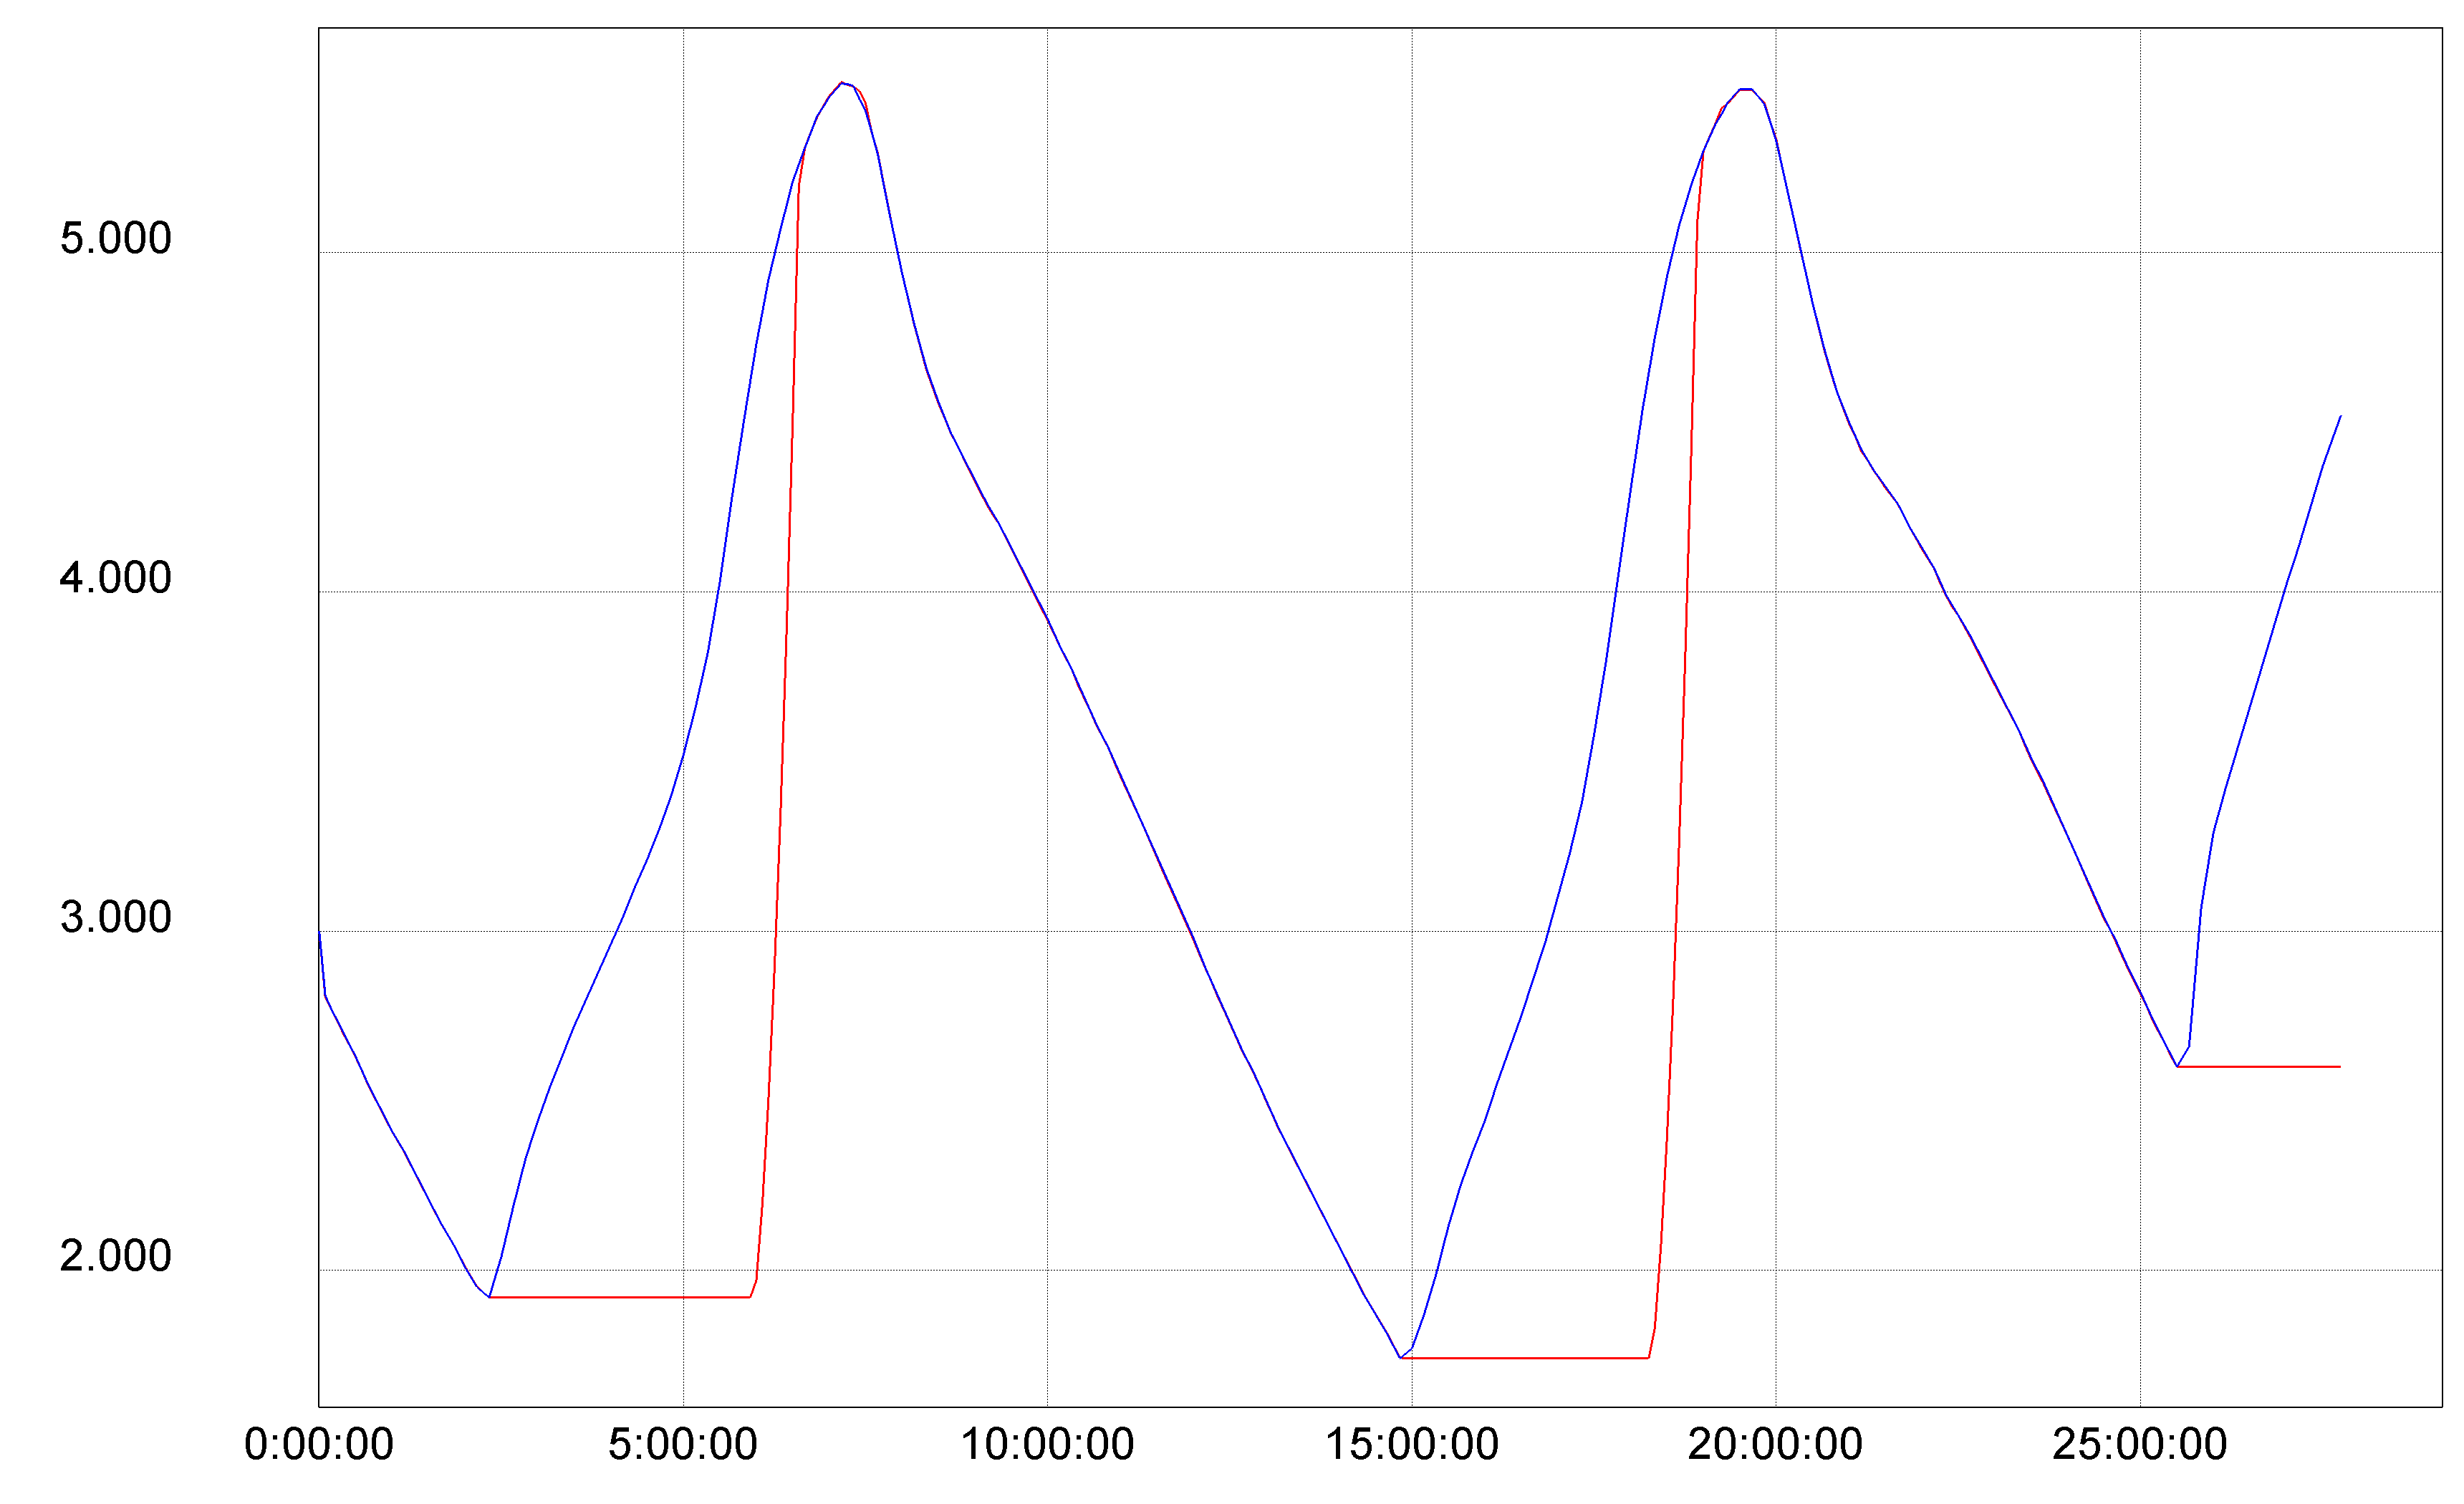
\includegraphics[scale=0.14]{img/figure2.png}
\end{center}
\caption{Schematic culvert test case : results of two tidal cycles.
The blue line gives the water level in the estuarine river part and the red line gives the water level in the floodplain.}
\label{fig:culvert_figure2}
\end{figure}

Figure \ref{fig:culvert_figure2} shows the results of a short simulation with the schematic scenario.
The blue line gives the water level in the estuarine river part and the red line gives the water level in the floodplain.
From the characteristics of the two culverts we can see that only culvert 1 allows flow in both directions (CLP=0)
and the base level of this culvert (max(z1,z2)) is at 4.7m.
In Figure \ref{fig:culvert_figure2} we see that the flow in the floodplain only starts when the water level in the estuary has reached 4.7m.
Because of the small scale of the schematic model and the real life characteristics of the culverts the outflow
of water out of the floodplain follows the estuarine water level one on one.

%\section{References}
